\section{CI / CD}

\frame{\tableofcontents[currentsection]}

\begin{frame}
    \frametitle{\href{https://circleci.com/blog/what-is-continuous-integration}{What is Continuous Integration?}}   
    \begin{itemize}
        \item Multiple developers pushing small, frequent changes to a shared repository
        \item Often comes with Continuous Deployment
        \item CircleCI build has generally multiple steps:
        \begin{itemize}
            \item dependencies
            \item testing
            \item deployment
        \end{itemize}
    \end{itemize}
\end{frame}

\begin{frame}
    \frametitle{How your repo will look like}   
    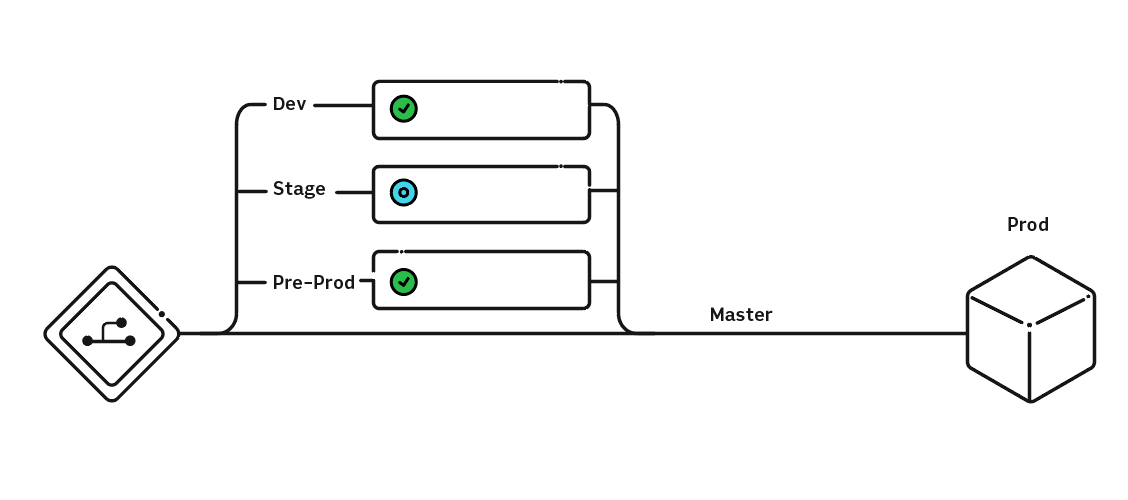
\includegraphics[scale=0.25]{01-sample-branches}
    
    feel free to simplify this to following branches:
    \begin{itemize}
        \item dev
        \item prod
    \end{itemize}
    You can configure your CI/CD to do specific task on specific branches (e.g. only deploy prod branch)
\end{frame}
